So taking the first one, we had to study performance to cost of three solutions and their scalability:
    \begin{itemize}
        \item RDS (SQL)
        \item DynamoDB (NoSQL)
        \item Aurora (SQL)
    \end{itemize}

As all three were AWS solutions, the performance of each was pretty much the same,
and as the database was going to be used for archival it relied less on having a
high throughput and more on how much storage costs.
So we only relied on the cost of the solution, how easy is it to maintain.

So going off by cost first Aurora was the most expensive, with no value added to the problem we'll be solving with it.

So that left us with two options:
    \begin{itemize}
        \item RDS (SQL)
        \item DynamoDB (NoSQL)
    \end{itemize}

We dived into the RDS solution, and it was a bit of a challenge to get it to scale,
in terms of storage compared to DynamoDB which offered autoscaling options and variable
throughput for high load time which could fit the needs of archival as it could take 
higher input in the daily backup process, than the rest of the day.
And for the output there wasn't much to be gained, for neither of the solutions as it was
a rare process that wouldn't be used alot only on demand by the user.

Going to studying the cost, the primary tool that was used for that is the AWS Cost Calculator, which gives rather good indicators to approximate the charges.

\textbf{Case study: }

For the data we used the following:
- 200 Entries per site.
- 500 Site.
- 2 KB per entry.

Site represents the factories and the entries represents the trucks.

So with those inital values, we came to the following results:
- Daily storage of 200 MB or monthly of 6 GB that increments after the period passes.
- 3000000 writes / month
- 100000 reads / month

the reads were just second guessed as there was no significant data about it, 
other than it will be a low read database.

So for the calculations, for RDS we used the following options:
- Instance db.t3.large (vCPU: 2 Memory: 8 GB)
- Instance reserver for one year 
- Single-AZ (1 node)
- 6 GB storage incremented monthly
- 6 GB backup incremented monthly

which resulted in the yearly cost of \$1185.769

For DynamoDB, we used the following options:
- Standard-Infrequent Access (Reduces cost of storage)
- 3 Mil writes per month
- 100K reads per month
- 6 GB storage incremented monthly
- 6 GB backup incremented monthly

Which came down to the cost of \$236.00 per year.

As we can notice the RDS cost was much higher than DynamoDB,
so we decided to use DynamoDB as it was cheaper, and also had
better maintenance options offered by AWS as it's a fully hosted
service.

Lastly, the only missing part was integration within the back-end which went on different steps.

First we had to create a service on the Spring Back-end that took on the handling of the communication layer between the DB and the back taking on mulitple functionalities such as:
    \begin{itemize}
        \item Creating - delete tables
        \item Creating indexes to allow fast access to the data
        \item Adding - deletting data
        \item Finding data using specific fields
    \end{itemize}

Then implementation of unit tests for the service to ensure that it's working as intended,
it had taken on the following tests:
    \begin{itemize}
        \item Create table for tests with required indexes
        \item Adding data to table, and then finding it
        \item Adding data to table, and find it by date
        \item Adding data to table, and find it by different keys
        \item Cleaning up the table
    \end{itemize}

The creation of the tables and their indexes was automated, to allow for the
reproduction of the same environment for the data we had during testing, and in the 
dev environment. Also, getting rid of the need for manual creation of the tables.

\begin{figure}[!htb]
    \centering
    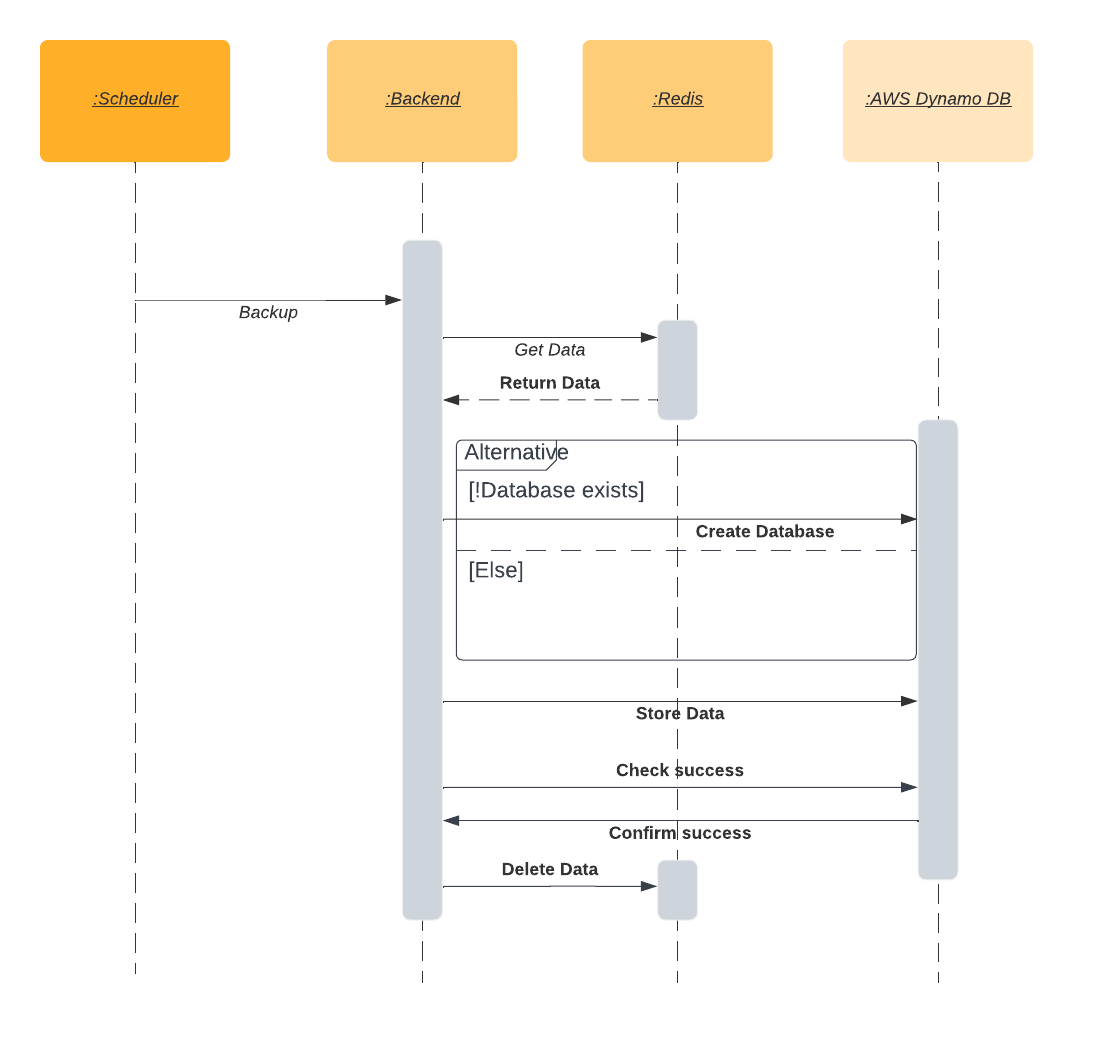
\includegraphics[width=0.8\textwidth]{images/archival_backup.png} 
    \caption{\footnotesize{Archival Cronjob - Sequence Diagram}}
    \label{fig:archival_backup}
\end{figure}

Finally the archival process came as a cronjob shown in figure \ref{fig:archival_backup},
that would take the data each day at 00:00 and archive it from the redis database to the
DynamoDB while checking that everything was successfully archived before cleaning the data
from Redis.

